\section*{Methods}\label{sec11}

In the following, we will describe the details of our proposed RL scheduling method.

\subsection*{GridSim environment}
In the GridSim environment, a provincial power grid with a high proportion of renewable energy is provided. The power grid consists of 126 buses, 185 transmission lines, 91 loads, and 54 generators. The power grid is described by an AC circuit model, and GridSim employs the power flow function to solve the coupled dynamics.

GridSim considers all the operational constraints that are present in real-world power scheduling scenarios.
In the case of generator startup/shutdown constraints, a thermal unit is allowed to be shutdown if reaching its minimum power in the last step, and then not allowed to be restarted in the next 40 steps, corresponding to the cooling process in the real world. If a thermal generator is restarted, it is not allowed to be shut down for the next 40 steps. 
For line outages, the disconnected lines are not allowed to be reconnected for 16 steps, corresponding to the maintenance period. 
Additionally, thermal generators have power ramping constraints due to their rotational inertia, which limits power changes within a single step. 

\subsubsection*{Reward design}
The reward function is crafted to provide guidance to the agent for compliance with the operational constraints and improvements on optimization objectives.
In accordance with the objectives and constraints of the RTS problem setting, the reward function is divided into distinct components.

\bmhead*{Line overflow.} 
To ensure the security of power transmission, we establish a reward mechanism that takes into account the current load rates of transmission lines. The current load rate is defined as the ratio of the transmission current to the maximum transmission current, which is limited by the thermal capacity of the line. 
To prevent line congestion and outages, it is desirable for the transmission lines to maintain a reasonable load level. Consequently, we design the reward function for this aspect as follows:
\begin{equation}
    r_{\text{overflow}}=1-\frac{\sum_i\min(\rho_i,1)}{n_{\text{line}}}
\end{equation}
where $\rho_i$ indicates the current load rate of line $i$. $n_{\text{line}}$ represents the line number. 

\bmhead*{Renewable consumption.} 
To optimize the utilization of renewable energy, a reward function is formulated to encourage the scheduling agent to consume more renewable energy. This reward function is based on the renewable energy consumption rate, which is defined as the ratio of the total power currently consumed from renewable sources to the maximum power generated by renewable sources. A higher renewable energy consumption rate corresponds to a higher reward, thereby incentivizing the agent to maximize the use of renewable energy. This reward is designed as follows:
\begin{equation}
    r_{\text{renewable}}=\frac{\sum_i\text{p}_i}{\sum_i\text{p}_i^{\text{max}}},\quad i\in\text{renewable units}
\end{equation}
where $\text{p}_i$ represents the power output of generator $i$, $\text{p}_i^\text{max}$ indicates maximal power generation capability of renewable generator $i$. The closer $\text{p}_i$ and $\text{p}_i^\text{max}$ are, the higher the renewable consumption reward.

\bmhead*{Balanced generator.} The balanced generator is to balance the residual power and eliminates discrepancies between power generation and load consumption, while its control capability is limited. If its power output exceeds its operational boundaries, a power mismatch occurs, which may result in load shedding or blackouts as previously mentioned. To prevent such failures and maintain safe operation, we design the reward function as follows:
\begin{gather}
    r_\text{balance} = -\left(\frac{\max(\text{p}_\text{bal}-\overline{\text{p}_\text{bal}},0)}{\overline{\text{p}_\text{bal}}-\underline{\text{p}_\text{bal}}}+\frac{\max(\underline{\text{p}_\text{bal}}-\text{p}_\text{bal},0)}{\overline{\text{p}_\text{bal}}-\underline{\text{p}_\text{bal}}}\right)
\end{gather}
where $\overline{p_\text{bal}}$ and $\underline{p_\text{bal}}$ indicate the upper bound and the lower bound of the balanced generator's active power. If the balanced power $p_\text{bal}$ is out of bounds, there would be a penalty.

\bmhead*{Operating cost.} We formulate a reward function for the operational costs of thermal units while considering the negligible costs of renewable energy generation. Specifically, the operating costs of thermal units are represented as quadratic functions of output power, and additional costs are incurred for the startup/shutdowns of thermal units. As for renewable sources, their operating costs are considered to be negligible as they do not rely on fossil fuels for power production. 
The operating cost reward is designed as follows:
\begin{equation}
    r_\text{cost} = -\frac{\sum_i c_{i,2}\text{p}_i^2+c_{i,1}\text{p}_i+c_{i,0}+\mathcal{I}(\text{s}_i, \text{s}_i^-)c_{\text{on-off,i}}}{Z}
\end{equation}
where $c_{i,2},c_{i,1}$ and $c_{i,0}$ are the second order, first order and constant coefficients of the operation cost of generator $i$, respectively. The coefficients of renewable units are much lower than that of thermal units. $\text{p}_i$ represents the power output of generator $i$. $\text{s}_i$ represents the on-off status of generator $i$, and the $\text{s}_i^-$ is the status 1-step advance. $c_\text{on-off,i}$ is the startup and shutdown costs of generator $i$. $\mathcal{I}(\text{s}_i, \text{s}_i^-)$ is an indicative function that turns to be 1 if $\text{s}_i\neq\text{s}_i^-$, otherwise 0. $Z$ is the normalization factor set as $10^5$ in experiments.

\bmhead*{Reactive power.} Reactive power plays a vital role in supporting the voltage stability of the power grid. However, the reactive power output capacity of the generators is constrained. While exceeding this limit is not catastrophic, excessive reactive power compensation can significantly increase operational cost. In light of these considerations, we design 
the reactive power reward as follows:
\begin{equation}
    r_\text{reactive}=\exp\left(-\sum_i\left[\frac{\max(\text{q}_i-\overline{\text{q}_i},0)}{\overline{\text{q}_i}-\underline{\text{q}_i}}+\frac{\max(\underline{\text{q}_i}-\text{q}_i,0)}{\overline{\text{q}_i}-\underline{\text{q}_i}}\right]\right)-1
\end{equation}
where $\text{q}_i$ is the reactive power of generator $i$, and $\overline{\text{q}_i}, \underline{\text{q}_i}$ are the upper bound and the lower bound of generator $i$. There would be a penalty if any generator violates its reactive power constraint. 

\bmhead*{Bus voltage.} In power system operation, it is common practice to limit node voltage magnitudes within the range of 0.95-1.05 per unit. If the voltage magnitude at a node is too low, it can result in a significant increase in the transmission loss of the grid. Conversely, if the node voltage magnitude is too high, it requires more reactive power compensation and may cause the generator's reactive power to exceed its upper limit.
To regulate the node voltage magnitudes within specified ranges, we design the bus voltage reward similarly to the reactive power reward.
\begin{equation}
    r_{\text{voltage}}=\exp\left(-\sum_i\left[\frac{\max(\text{v}_i-\overline{\text{v}_i},0)}{\overline{\text{v}_i}-\underline{\text{v}_i}}+\frac{\max(\underline{\text{v}_i}-\text{v}_i,0)}{\overline{\text{v}_i}-\underline{\text{v}_i}}\right]\right)-1
\end{equation}
where $\text{v}_i$ is the voltage magnitude of bus $i$, and $\overline{\text{v}_i}, \underline{\text{v}_i}$ are the upper bound and the lower bound of voltage magnitude of bus $i$. There would be a penalty if any bus violates its voltage magnitude constraint. 

The total reward is calculated as the weighted sum of the above reward parts.

\subsection*{GridZero}
Complex action spaces are common indeed in real-world problems, and so is the real-time scheduling (RTS) problem. The RTS problem requires the RL agent to make decisions simultaneously on optimal power outputs and generators' startup/shutdown. 
This section outlines the combination of Sampled MuZero~\cite{hubert2021learning} and EfficientZero~\cite{ye2021mastering} to develop the core GridZero algorithm for solving the online control of RTS.  
To provide a better understanding of our work, we use Fig.\ref{fig:how_gridzero_work} to demonstrate how GridZero performs planning, acting, and training.

\begin{figure}[h]
  \centering
  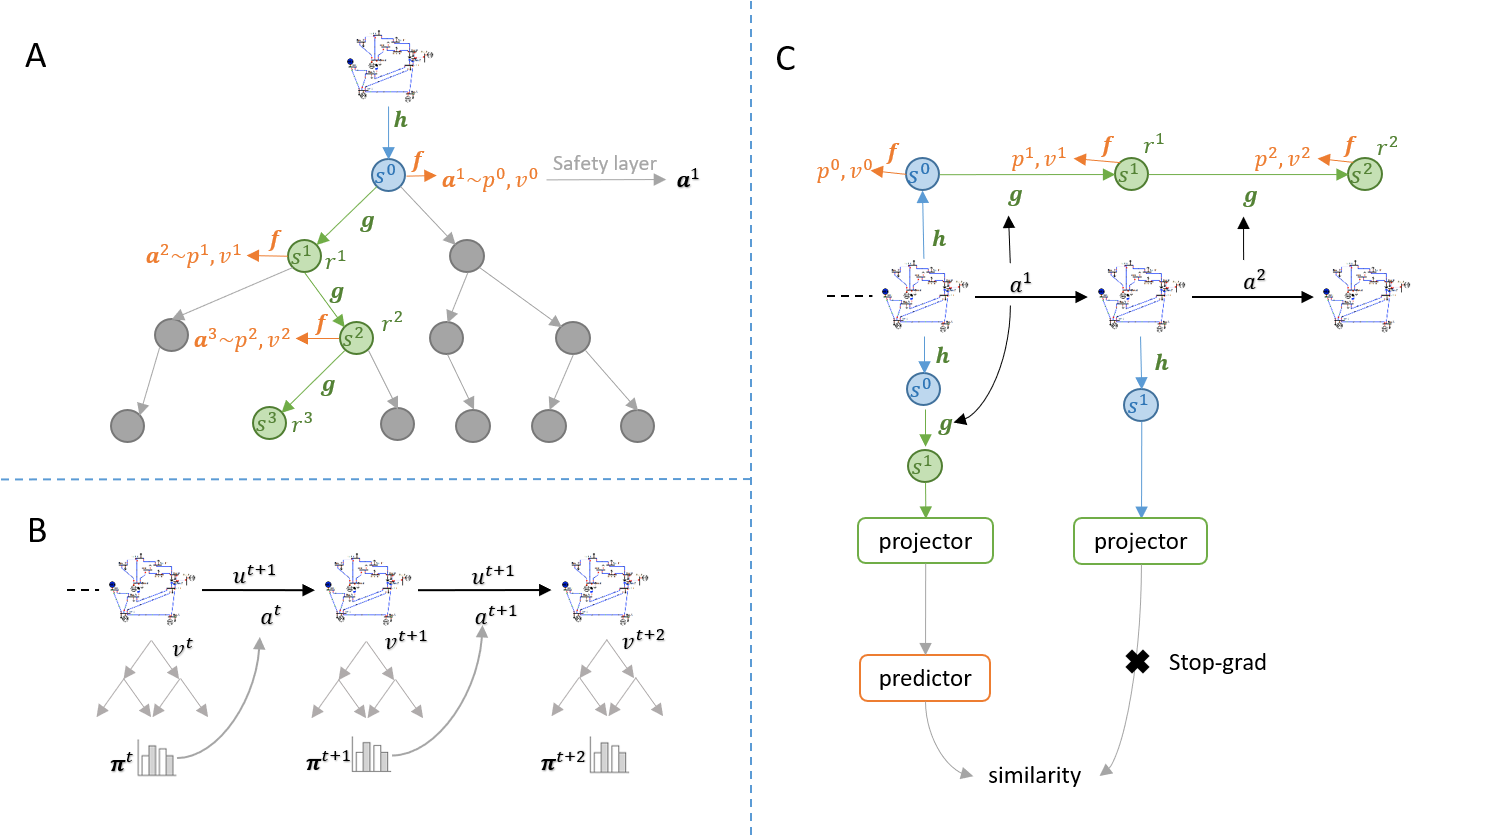
\includegraphics[width=1.0\linewidth]{fig/birdsight_gridzero_v2.png}
  \caption{\textbf{Planning, acting, and training of GridZero.} \textbf{(A) Planning.} The model includes representation $h$, dynamics $g$, and prediction function $f$. The dynamics network $g$ predicts the reward $r^t$ and the next hidden state $s^t$ when given a hidden state $s^{t-1}$ and action $a^t$. The prediction network $f$ computes the policy $p^t$ and value estimation $v^t$ using $s^t$. Action candidates $\{a^t_i\}$ are sampled from $p^t$, with root action candidates processed by the safety layer. The representation network $h$ embeds the hidden state $s^t$ using the observation of power grid $o^t$. \textbf{(B) Acting.} An MCTS tree is expanded at each step $t$. An original action $a^{t+1}$ is sampled from the visit count distribution $\pi^t$, mapped to a real action $\tilde{a}^{t+1}$ by the action mapping layer, and then used to simulate a new observation $o^{t+1}$ and return a ground-truth reward $u^{t+1}$. \textbf{(C) Training.} The model is unrolled for $K$ steps.
  At each step $k$, the dynamics network $g$ receives $s^{k-1}$ and the action $a^{k}$ as input, generates the next hidden state $s^{k}$ and reward estimation $r^{k}$. GridZero learns by mimicing the policy $p^{k}\to\pi^{k}$, value estimation $v^{k}\to z^{k}$, and reward estimation $r^{k}\to u^{k}$, where $z^{k}$ is the bootstrap prefix value target. GridZero also introduces a consistency loss by using the self-supervised network to calculate the similarity between the estimated hidden state $\hat{s}^{k+1}$ and the target hidden state $s^{k+1}$.}
  \label{fig:how_gridzero_work}
\end{figure}

We first present the sampling method and the hybrid policy, which allows GridZero to accommodate to the hybrid action space of power scheduling, consisting of both discrete startup/shutdowns and continuous power outputs. 
Action candidates for MCTS are sampled from the hybrid policy $p$, which includes a continuous power adjustment vector and startup/shutdown one-hot vectors. 
In MCTS, the agent selects the action of the child with with the highest Upper Confidence Bound (UCB) score to visit, which is formulated as
\begin{equation}
    a=\mathop{\arg\max}\limits_{a\sim p}Q(s,a)+\hat{\beta}(s,a)\frac{\sqrt{\sum_b N(s,b)}}{1+N(s,a)}
\end{equation}
The hybrid policy $p$ consists of a Gaussian distribution corresponding to the continuous policy and a categorial distribution corresponding to the discrete policy. $Q(s,a)$ and $N(s,a)$ is the Q-value estimation and visit count of state-action pair $(s,a)$. $\hat{\beta}(s,a)$ is a uniform prior distribution in GridZero's setting. 

In order to train GridZero, the loss function is formulated as
\begin{equation}
    l=\sum_{k=0}^K l^r(u^{k},r^{k})+l^v(z^{k},v^{k})+l^p(\pi^{k},p^{k},\bm{a}^k)+l^c(s^{k+1},\hat{s}^{k+1})+H(p^{k})
    % +c\Vert\theta\Vert^2
\end{equation}
The loss function is computed over a horizon of $K$ unrolled steps. The reward loss $l^r$ measures the difference between the estimated reward $r^k$ and target reward $u^{k}$. Similarly, The value loss $l^v$ indicates the difference between the estimated value $v^k$ and bootstrapped target value $z^{k}$. The policy loss $l^p$ represents the distance between the output policy $p^k$ and the target root visit distribution of MCTS $\pi^{k}$, and $\bm{a}^k$ is the root action candidates at step $k$.
In order to address the challenge of insufficient supervisory signal in dynamic networks in MuZero, we introduce consistency loss $l^c$ which maximizes the similarity between the predicted next-state $\hat{s}^{k+1}$ and the target next-state $s^{k+1}$ derived from the observation $h(o^{k+1})$. Additionally, we incorporate the entropy loss term $H(p^{k})$, following the SAC's settings, to encourage exploration in the learning process\cite{haarnoja2018soft}. 

\subsubsection*{Hybrid Action Sampling}
To more accurately represent the power output adjustment and switching behaviors of generators, we utilize a hybrid action that concatenates a continuous vector in the range of $[-1,1]^n$ with two one-hot vectors $\left\{0,1\right\}^{n+1}$, representing the control of active power and startups/shutdowns of generators, respectively.

In brief, the output of the policy network is now split into four parts: Gaussian means $p_\mu$, Gaussian logarithmic standard deviations $p_\sigma$, discrete startup logits $p_o$ and discrete shutdown logits $p_c$. The dimensions of $p_o$ and $p_c$ are both $n+1$, where $n$ is the number of generators, with the additional dimension corresponding to no startup or shutdown. The active power control vector $a_p$ is generated by sampling from a squashed multivariate Gaussian distribution $\overline{\mathcal{N}}(p_\mu, p_\sigma)$. The one-hot vectors of startups $a_o$ and shutdowns $a_c$ are sampled from categorial distributions $p_o$ and $p_c$. An action candidate $a_i$ of the root is the concatenation of $a_p$, $a_o$ and $a_c$. The candidates of root nodes are required to be corrected by the safety layer since random exploration is not allowed in this security-constrained task. Our action mapping layer only maps the selected root action candidate $a$ to a practical action as follows:
\begin{equation}
    \tilde{a} = 
    \frac{a_\text{p}-(-1)}{1-(-1)}
    % \frac{a_\text{p}+1}{2}
    \cdot(\overline{\text{p}}-\underline{\text{p}})+\underline{\text{p}}+\overline{\text{p}}\cdot a_o+\underline{\text{p}}\cdot a_c
\end{equation}
where $\overline{\text{p}}, \underline{\text{p}}$ are the time-varying upper bound and lower bound of the action space, $[a_p, a_o, a_c]$ is the original sampled action, including active power control, startup/shutdown one-hot vectors.


\subsubsection*{Design of Power Balancing Safety Layer}
Exploration without violations to constraints is a critical challenge in our problem. This is because not all states are accessible, particularly those that may result in severe consequences. 
The RTS problem has complex operational constraints, however, the most crucial constraint is power balancing, which requires that the power generation be equal to load consumption at any time.
The fluctuating loads and renewable generation introduce temporal variations into the power balancing constraint, which makes it more difficult to maintain this constraint.
We found that simple reward shaping and auxiliary loss methods cannot solve this problem since the action space is high-dimensional and time-varying. 

Therefore, We propose a safety layer to ensure that the agent satisfies this basic power balancing constraint, which is equivalent to restricting the feasible solution space. 
The safety layer calculates the readjustment power $\Delta a$ through two objectives, balancing the predicted change in total load $\Delta\hat{\text{p}}_{\text{load}}=\hat{\text{p}}^{t+1}_\text{load}-\text{p}^t_\text{load}$, and 'pulling' the deviated balanced generator power back to its safe range $[\underline{\text{p}_{\text{bal}}}+\delta, \overline{\text{p}_{\text{bal}}}-\delta]$.
With this information, we calculate a readjustment objective $\Delta a$ for other generators using the following equation:
\begin{equation}
\label{eq:safety_obj}
    \Delta a=\Delta\hat{\text{p}}_{\text{load}}-\sum_i \tilde{a}_i+\Delta \text{p}_{\text{bal}}
\end{equation}
where 
\begin{equation}
    \label{eq:safety_pbal}
    \Delta \text{p}_{\text{bal}}=
    \left\{
             \begin{array}{lr}
             -(\overline{\text{p}_{\text{bal}}}-\delta-\text{p}_{\text{bal}}), & if\ \text{p}_{\text{bal}}>\overline{\text{p}_{\text{bal}}}-\delta \\
             \text{p}_{\text{bal}}-\underline{\text{p}_{\text{bal}}}-\delta, & if\ \text{p}_{\text{bal}}<\underline{\text{p}_{\text{bal}}}+\delta. 
             \end{array}
\right.
\end{equation}
with $\delta$ as the redundancy to the limits. $a_i$ refers to the power adjustment of generator $i$. 
% Once the overall readjustment target $\Delta a$ is derived, we calculate the adjustment for each unit to form the feasible action. 
The readjustment target $\Delta a$ will be allocated to each online generator in proportion. The allocation proportion is determined by the generator's climbing capacity. The lager the climbing capacity, the greater the allocation power.
The closed generators are supposed to be masked out because they are not adjustable. We only readjust those adjustable units if the objective $\Delta a$ exceeds a threshold, which means that the safety layer is not always active. This is because we want to enable the agent reasonable exploration space, as long as it is within the power balancing constraint.  In our experiments, the threshold is a number smaller than the redundancy $\delta$. 
We can calculate the readjustment of each generator as follows:
\begin{equation}
\label{eq:safety_readj_value}
    \Delta a_{i}=
    \left\{
             \begin{array}{lr}
             \Delta a\cdot(\overline{\text{p}_i}-a_i)/\sum_i(\overline{\text{p}_i}-a_i), & if\ \Delta a>0 \\
             \Delta a\cdot(a_i-\underline{\text{p}_i})/\sum_i(a_i-\underline{\text{p}_i}), & if\ \Delta a\leq 0. 
             \end{array}
\right.
\end{equation}
so the legalized action turns to be $a_i=a_i+\Delta a_i$. 

Such a safety layer essentially maps the original action space of the policy network output to a time-varying feasible solution space, which satisfies the fundamental power balancing constraint. 

\subsubsection*{Exploration noises on root nodes}

To ensure enough exploration to approach a near-optimal control policy, we propose two types of noises for both continuous active power control and discrete switching actions. 
For discrete actions, we introduce Dirichlet noises to the switching probabilities, resulting in the one-hot vectors being sampled from the perturbed categorical distribution. Regarding continuous actions, we consider two approaches. The first approach is to add standard normal noises to the sampled actions, which can result in more radical explorations. The second approach involves sampling from a more flattened Gaussian by doubling the variance, as in $\bar{\mathcal{N}}(p_\mu, kp_\sigma)$, thereby leading to conservative explorations around the current policy. Finally, we use a mixture of the above methods:
% First, we add Dirichlet noises to the switching probabilities for discrete actions, and then the one-hot vectors are sampled from the disturbed categorial distribution. One approach for continuous actions is adding standard normal noises to sampled actions, which might produce more radical explorations. Another approach is to sample from a more flattened Gaussian by doubling the variance like $\bar{\mathcal{N}}(p_\mu, kp_\sigma)$, leading to conservative explorations in the vicinity of the current policy. Finally, we use a mixture of the above as follows:
\begin{equation}
    a=
    \left\{
             \begin{array}{lr}
             \sim\mathcal{N}(p_\mu, p_\sigma), & \text{sample $K_{\text{normal}}$ actions} \\ 
             \sim\mathcal{N}(p_\mu, p_\sigma)+\mathcal{N}(0,1), & \text{sample $K_{\text{bigger}}$ actions} \\
             \sim\mathcal{N}(p_\mu, kp_\sigma), & \text{sample $K_{\text{smaller}}$ actions}
             \end{array}
    \right.
\end{equation}
where total action candidates number is $K=K_{\text{normal}}+K_{\text{bigger}}+K_{\text{smaller}}$. In self-play, all the disturbed sampled actions of the root node should be processed by the safety layer.

\subsubsection*{Policy loss for hybrid actions}
To suitably tailor GridZero to accommodate a complex action space, we have implemented certain alterations to GridZero's policy loss. 
Within our hybrid action sampling, an action candidate $a$ is comprised of concatenated power adjustments $a_p$, startup binary one-hot encoding $a_o$, and shutdown binary one-hot encoding $a_c$. Concerning the continuous aspect of this framework, the loss function is represented as the Kullback-Leibler(KL) divergence of root distribution and policy distribution, as exemplified in Eq.\ref{eq:policy_loss_continuous}.
\begin{equation}
\label{eq:policy_loss_continuous}
    l^p_c=-\pi^\top\log p(a_p)
\end{equation}
where $a_p$ is the action candidate sampled from Gaussian policy $p(\cdot)=\mathcal{N}(p_\mu,p_\sigma)$. $\pi$ is the visit count distribution of the MCTS root node. In the case of discrete actions, we sample a limited number of actions because there are numerous possible combinations of generator switches. If all the combinations were taken into account, it would affect the search efficiency of MCTS. Nonetheless, this will introduce a dimension mismatch between the discrete policy distribution and the root visit distribution. To address this mismatch, we perform dot production of visit priors and one-hot actions as $\pi\cdot a_o$, which serves as the target switching policy. The loss function for the discrete policy loss is given by:
\begin{equation}
    l^p_d=-(\pi\cdot a_o)^\top \cdot\text{LogSoftmax}(p_o)-(\pi\cdot a_c)^\top\cdot\text{LogSoftmax}(p_c)
\end{equation}
where $p_o$ and $p_c$ are policy logits for units' startup/shutdown. $a_o$ and $a_c$ are target startup and shutdown actions. The total policy loss is a combination of continuous part and discrete part:
\begin{equation}
    l^p=l_c^p+l_d^p
\end{equation}

